\documentclass[tikz,border=8pt]{standalone}
% Shared look for every TikZ diagram. Load with \input{../../tools/tikz-style.tex}
\usepackage[T1]{fontenc}
\usepackage{lmodern}
\renewcommand{\sfdefault}{lmr}  % diagrams use the same serif as the text
\usetikzlibrary{arrows.meta, positioning, shapes.geometric, calc, fit, backgrounds}
\definecolor{cblue}{HTML}{4C78A8}
\definecolor{corange}{HTML}{F58518}
\definecolor{cgreen}{HTML}{54A24B}
\definecolor{cred}{HTML}{E45756}
\definecolor{cpurple}{HTML}{B279A2}
\definecolor{cgrey}{HTML}{6B6B6B}
\tikzset{
  every picture/.style={font=\sffamily, line width=1.2pt},
  box/.style={draw=#1, fill=#1!12, rounded corners=4pt, align=center, inner sep=7pt, minimum height=1.1cm},
  box/.default=cgrey,
  arrow/.style={-{Stealth[length=3mm]}, draw=cgrey, line width=1.4pt},
  title/.style={font=\sffamily\bfseries\Large},
  note/.style={font=\sffamily\small, text=cgrey, align=center},
}
\AtBeginDocument{\hyphenpenalty=10000 \exhyphenpenalty=10000}

\begin{document}
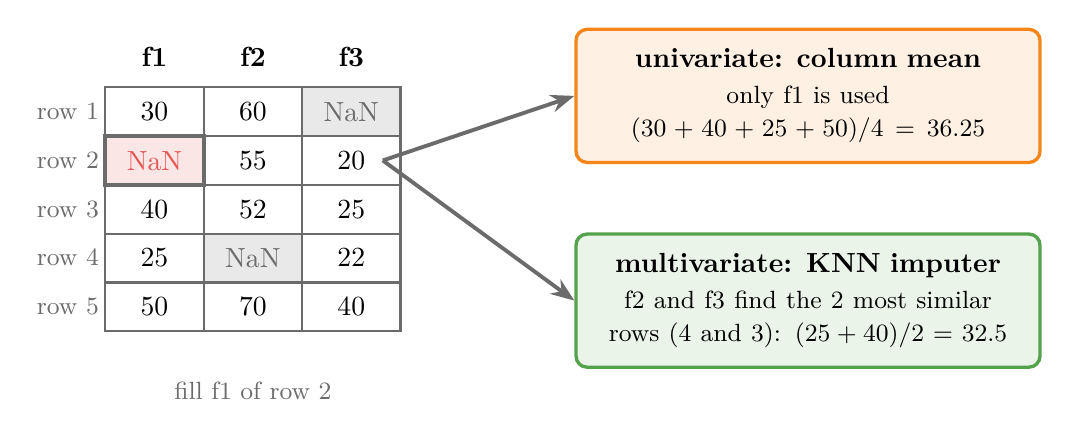
\begin{tikzpicture}[cell/.style={draw=cgrey, line width=0.8pt, minimum width=1.25cm, minimum height=0.62cm, font=\sffamily}]
  % the table with one gap
  \foreach \c/\h in {0/f1, 1/f2, 2/f3} \node[font=\sffamily\bfseries] at (1.25*\c,0.7) {\h};
  \foreach \r/\a/\b/\cc in {1/30/60/NaN, 2/NaN/55/20, 3/40/52/25, 4/25/NaN/22, 5/50/70/40} {
    \node[note] at (-1.1,-0.62*\r+0.62) {row \r};
    \foreach \v [count=\c from 0] in {\a,\b,\cc} \node[cell] (c\r\c) at (1.25*\c,-0.62*\r+0.62) {\v};
  }
  \foreach \p in {c12, c41} \node[cell, fill=cgrey!15, text=cgrey] at (\p) {NaN};
  \node[cell, fill=cred!15, text=cred, line width=1.4pt] at (c20) {NaN};
  \node[note, text width=4.2cm] at (1.25,-3.55) {fill f1 of row 2};
  % univariate
  \node[box=corange, text width=5.4cm] (uni) at (8.3,0.2) {\textbf{univariate: column mean}\\[2pt]\small only f1 is used\\ $(30+40+25+50)/4 = 36.25$};
  % multivariate
  \node[box=cgreen, text width=5.4cm] (mul) at (8.3,-2.4) {\textbf{multivariate: KNN imputer}\\[2pt]\small f2 and f3 find the 2 most similar\\ rows (4 and 3): $(25+40)/2 = 32.5$};
  \draw[arrow] (2.9,-0.62) -- (uni.west);
  \draw[arrow] (2.9,-0.62) -- (mul.west);
\end{tikzpicture}
\end{document}
